\section{メッセージの初期化と更新順序}
ここで,上記メッセージの初期化と更新順序について明記しておく.初期値について表\ref{tb:init_Message}に示す.
\begin{table}[htb]
	\begin{center}
		\caption{メッセージの初期値\label{tb:init_Message}}
		\begin{tabular}{|c|c|} \hline
			$\hat{x}_{kt}$ & pilot信号・・・$x$と同値,その他・・・0 \\ \hline
			$\xi_{kt}$ & pilot信号・・・0 その他・・・1 \\ \hline
			$\overline{x}_{kt}$ & pilot信号・・・$x$と同値,その他・・・0 \\ \hline
			$\overline{\xi}_{kt}$ & 1 \\ \hline\hline
			$\hat{h}_{nk}$ & 0\\ \hline
			$\eta_{nk}$ & 1\\ \hline\hline
			$\overline{I}_{nt}$ & 0\\ \hline
			$\zeta_{nt}$ & 0\\ \hline
		\end{tabular}
	\end{center}
\end{table}

計算順序について,図(\ref{fig:flow_message})にフローチャートを示す.
\begin{figure}[htbp]
  \begin{center}
    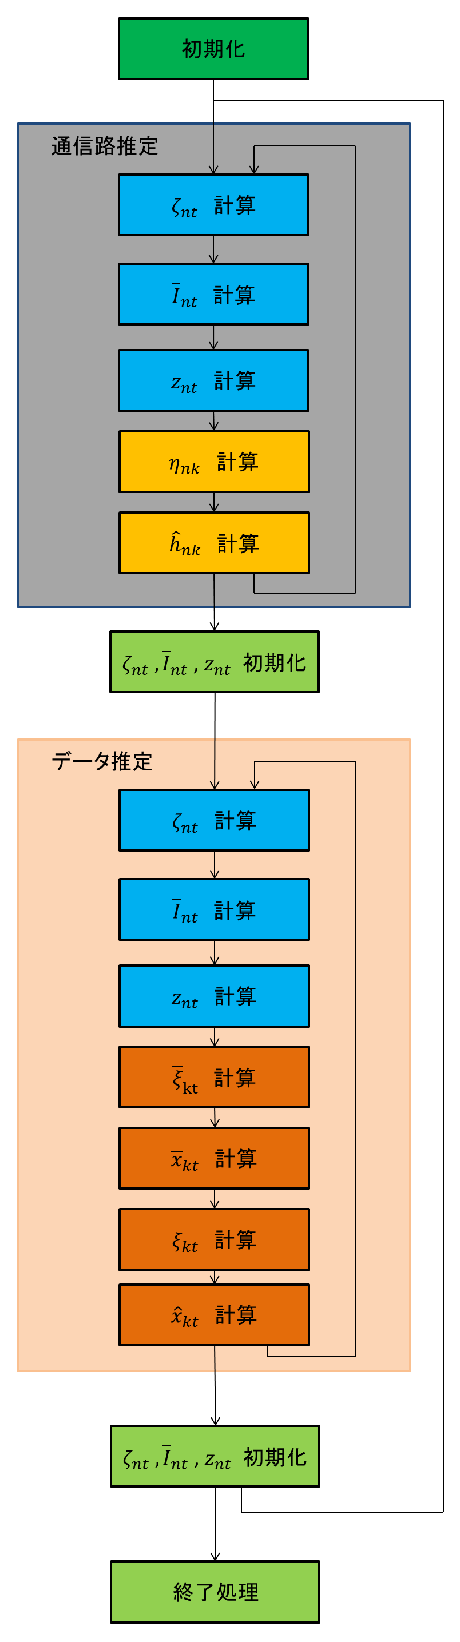
\includegraphics[clip,width=5.0cm]{./flow_message.eps}
    \caption{メッセージの計算順序}
    \label{fig:flow_message}
  \end{center}
\end{figure}